\cotefile{29}
\scanpage{3}
Voorschoten, May 16 1967.\\
Palestrinalaan 11.\\

Dear Grothendieck,\\

I am trying to work out your letter with indications. However I have many difficulties and my progress is very slow. Usually I could find out from your manuscripts for what purpose you developped things in such or such a way, but this time I doubt whether I have grasped the essential points. I can understand your set-up only against the lemma of Abhyankar as background, namely instead of \unsure{giv\deleted{e}ing|giv\deleted{i}eng} directly the covering $\underline{r}(X)$ (in your notation) of $S$, you give the ``behaviour'' of the covering over other coverings, namely the $\underline{s}(M)$, which are of a particular type; apparantly the behaviour over \unsure{a\deleted{l}al|a\deleted{a}ll} these $\underline{s}(M)$ together gives better information then the $\underline{r}(X)$ alone. Is this intuitively a reasonable way of thinking over your new set-up\handwritten{?}

My main difficulty is that I don't see that for a Galois covering the extra structure is uniquely determined. First the concept of Galois covering itself\rlap{\handwritten{\raisebox{.55ex}{.}}}. After the abstract definition and some var\inserted{\handwritten{i}}ations you write: ( I assume that you have a copy) On peut enfin l'expliciter en revenant \handwritten{\`}{a} la definition de $\mathrm{Rev}^{\underline{R}}(S)$, et en exigeant que les revêtements des $\underline{s}(M)$ correspondants \handwritten{\`}{a} $X$ soient principaux de groupe $G$. Now in all your examples there is also a group working on the $\underline{s}(M)$, for instance in example 1 a group $\handwritten{\unsure{\mathfrak{g}|g|\mathscr{G}}}$ working on $Z$, and this group acts also on the Galois covering \inserted{\handwritten{\unsure{Corresponding|corresponding} with}} $X$. It seems to me that one must require that the actions of $G$ and $\handwritten{\mathfrak{g}}$ commute\rlap{\handwritten{\raisebox{.55ex}{.}}}, is this correct\handwritten{?} On the same and the next page of your letter you \unsure{explai\deleted{n}m|explai\deleted{m}n} (for example 1) that the functor $\underline{r}$ (geometric realization) is fully faithful (restricted to Galois coverings) under certain conditions; this I don't understand at all ( and \deleted{makes} this makes me feel very uncertain, since I expect that this is an important point \deleted{f} if \unsure{\deleted{o}wne|\deleted{w}one} wants to see what is going on\handwritten{!}).

Some other points\rlap{\handwritten{\raisebox{.55ex}{.}}}. in the final formulation of example 3 you introduce a sheme of groups $G(M)$\rlap{\handwritten{\raisebox{.55ex}{.}}}, \deleted{with this formulation} do the objects in example 3a ,with this formulation, consist\deleted{s} out of \uline{couples} $M=(\underline{a},\underline{n})$ and $G(M)=\handwritten{\mu}_{\underline{n}}$ \handwritten{?} Also you write\rlap{\handwritten{\raisebox{.55ex}{.}}}. $\mathrm{Hom}_{\handwritten{\unsure{s|S}'}}(M',M)$ est vide sauf si $\underline{n}'\handwritten{\geqslant}\underline{n}$, auquel cas....etc....., it seems to me that this sh\handwritten{\tikz[overlay,baseline]{\draw[line width=.4pt] (0,-.02) .. controls (.08,.23) and (.17,.25) .. (.20,.06) .. controls (.22,-.12) and (.36,-.15) .. (.39,-.02);}}uold be ....sauf si $\underline{n}'=\underline{m}.\underline{n}$, auquel cas..... and where $\underline{m}=(m_i)_{i\handwritten{\in}I}$is a a set of positive integers.

\margin{\handwritten{\unsure{,|'}}}
% archive sheet number: 2

\scanpage{4}
\mspage{2.}
I realize that I cause you a lot of trouble and work by asking every time for further explanation and that my assistance in writing the exposé is not very large. Therefore I suggest that you answer this letter only in case it is clear from my questions that I have really a misconception of your new set-up (and it would not surprise me if I have...). Otherwise I shall try to work out your theory as good as I can and make a preliminary manuscript which we can discuss when I am at Bures (I plan to come June 2). In any case, I hope to complete the definit\handwritten{e} version during my stay in Bures.

With kind regards,\\
Sincerely yours,\\
\handwritten{J.P. \unsure{Murre}}\\
% archive sheet number: 3

\scanpage{5}
Voorschoten, March 29 1967\\
Palestrinalaan 11\\

Dear Grothendieck,\\

Enclosed I send you - finally - ,in two different covers, the manuscript on the tame fund. group together with the papers which I borrowed from you.

As to the terminology: I have used scheme in stead of prescheme (without mentioning it, because I expect this will be \deleted{\unsure{f}}\inserted{a} general remark in SGA I) but I have not used ``doublet'' because I don't know your final decision on this point.
\margin{\figure{
\begin{tikzpicture}[scale=.8]\node[rotate=31] at (-.65,0) {stroke};\draw (.4,-.25)--(.4,.45);\end{tikzpicture}}}

References: I have made freely references to EGA (also to EGA IV) \uline{but only to SGA 1960/61} (with one notable misleading : a reference to SGA X, Cor 3.3 etc, the purity theorem, is a misleading because the proof is only in SGA 1962). I don't know the \unsure{`|``}new numbering' of SGA (You mentioned something about it, but I don't remember) so I have used still SGA I, SGA V etc for the 1960/61 séminaire.
\margin{SGA 1}

I must admit that there are still many points which are not satisfactory in the exposition. Below are some comments, motivations and questions:

p.3 Hyp.1\quad Perhaps it would have been nicer to avoid a little longer this assumption. However there is in SGA 1960/61 only a statement about quotients and existence of quotients in case the group is an \uline{ordinary} finite group (it is only in SGA D that the theorems from TDTE III are proved and the proof is long and subtle!) This is the reason for making the assumption Hyp 1 already here.

p.5. line 6 below:\quad the emphasis on $H$ ordinary group \unsure{.:|:} same reason

p.6 (Cor 1.11)\quad \uline{In fact this is a general question} : I have hesitated a little bit \unsure{W|w}ith the word ``covering'' for ``revêtement'' (of course: already used in the title!)
\margin{\figure{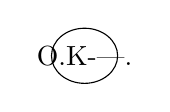
\begin{tikzpicture}[scale=.7]\draw (0,0) ellipse (.6 and .5);\node at (0,0) {O.K\unsure{-|.}};\end{tikzpicture}}}
Originally revêtement was used as translation \deleted{for covering} (in Serre\unsure{.|-}Lang's paper) for covering (in Lang's paper)!\unsure{.} But now there may be confusion with ``covering in some topology'' for instance ``covering in the étale topology'' which is something entirely different. What do you think about this? I don't see what
\margin{O.K.}
% archive sheet number: 4

\scanpage{6}
\mspage{2.}
word to use else.

\reversemarginpar
\margin{!}\uline{p.19 etc} : I expected lemma 4.3 to be almost trivial but when I tried to write a proof I did not see an easier one\deleted{\unsure{?}}. Also : the proof of lemma 4.4 is kind of subtle (but this could be expected).

p.26. line 1:\quad I shall try to find a precise reference.

line 3 :\quad the condition : irreducible in \uline{Zariski topology} is unpleasant but I have not been able to avoid it.

last line in 3) :\quad it seems necessary to mention also the points $s'$.

p.33,34 etc \unsure{..|:}\quad I did not see an easier proof for prop 7.4.

p.43 theor.9.4\unsure{.}\quad You have mentioned that the theorem in this form is not satisfactory . for instance the trivial case with constant fib\unsure{re|er}s and arbitrary crossings escapes. However I don't see how to get a satisfactory statement.

p.45. line 5 etc.\quad Is this indication sufficient?

I have not written an appendix on the Lefschetz theory. If you think this is useful then I can still try.
\margin{\figure{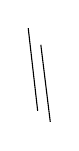
\begin{tikzpicture}\draw (0,1.05)--(.12,0);\draw (.16,.84)--(.28,-.14);\end{tikzpicture}}}
\normalmarginpar

It is not necessary to return the manuscript, I have a carbon copy so you can refer to pages and numbers in your comments. Please give me, if necessary, indications for the way the final manuscript must be typed (is the book a \deleted{foto} photo \unsure{C|c}opy of the manuscript?) Also give me a deadline when you must have the \unsure{M|m}anuscript because I am afraid that I may have already delayed the publication date of your first volume.

With best regards,\\
Sincerely yours,\\
J.P. Mu\unsure{rre}\\
% archive sheet number: 5

\scanpage{8}
Dear Murre,\\

Thank\deleted{\unsure{s|x}} you very much for your notes ont the tame fundamental group, which I at last finished reading. I see you wrote them with much care, and I am all the more sorry that \unsure{b|h}y my own fault, there is a number of misstatements which, I am affraid, will force you to do a serious recasting of the whole exposition. My notes definitely where too sketchy, and my oral explanations, I am affraid, partly wrong, which induced you into error a few times. Here the most serious drawbacks.

1.16. is false already when $H$ is the unit group and when there is a single $a$, say $a=b^n$, $Y'=Y\ T/(T^n-a)$. Then $Y=S$, and a morphism\deleted{\unsure{s|x}} of $Y$ into $Y'$ compatible with $H=e\quad H'$ is just a section\raisebox{-.45ex}{\deleted{\unsure{x|r}}} of $Y'$, which exists indeed; however $H\quad H'$ is not surjective. \unsure{3|\handwritten{3}}.6. is equally false, as you see by the previous example, using the given section to define an $H'$-morphism $H'\quad Y'$ which is not an isomorphism\rlap{\handwritten{\tikz[overlay,baseline]{\draw[line width=.5pt](-.03em,-.12ex)--(.36em,1.7ex);}}}. As a consequence, the proof in your notes of 3.7. breaks down (as it uses 1.16) and so does the proof of 3.8. (I did not try to check 3.8. by some different proof).
% Blank slots after Y, between H=e and H', between H and H', and between H' and Y' contain no visible brackets or arrows.
% The four reference 3s have the same angular top and curved lower part; typewriter-first state remains uncertain at the first occurrence.
% After isomorphism: a typed full stop is crossed/completed by a handwritten oblique stroke; the composite is exclamation-like.

I am affraid \deleted{the proof of} 6.4. is false as stated, and that the statement is correct only if the $D_i$ are regular. Indeed, the end of then \deleted{proo} proof seemed to me very dubious; be careful that the intertia groups are determined only up to interior automorphism ! There is however a \inserted{(tautological)} generalization of the theorem for regular $D_i$, corresponding to the data of a single divisor $D$ with normal crossings, and a variant of the notion of tame ramification for such a divisor, by demanding that the coverings should be tamely ramified locally fot the étale topology for the family of local irreductible components of $D$; it is this notion of tameness which would seem more adapted to the situation of par.9 .
% The cancelled line-end proo reaches the physical right edge; no final f is visible.
% archive sheet number: 7

\scanpage{9}
\normalmarginpar
\margin{\handwritten{\unsure{11/4/67|17/4/67|11.4.67|17.4.67}}}
The proof of 7.1. is not correct, when you conte\inserted{n}d on line -9: there remains to be proven the following: ... Already when $D=0$, the proof here would have to introduce conne\unsure{\deleted{f}c|\deleted{c}f}ted étale coverings which are \uline{not Galois} ! This very strongly suggests that a notion of tame ramification should be introduced also \deleted{in} for non Galois coverings. The same remark applies to the proof of 10.1. Maybe you could get along some way in 7.1. using the normali\deleted{\unsure{x|s}}ty assumptions, but I am convienced that these assumptions are anyhow artificial, as well as the assumption that the $D_i$ should be reduced somewhere. You do not seem to make any use of these facts, really
% The right paper edge follows the fully visible y of really; no terminal point is visible.

Also, one feels that 7.\unsure{\deleted{4}5|\deleted{5}4}. should be generalized to the case of a tamely ramified covering, and that it should come out trivially once the generalities have been dealt with properly.

I hope that the theory will come out more clearly and correctly by devoting some care to generalities on ramification data (not necessarily of Kummer type). I will try to write something up within the next days. Please excuse me for the trouble I caused you by not learning my lesson well enough before I put you to work !

It would be very nice indeed to have an appendix on Lefschetz theorem for the tame fundamental group, and it should not be hard to write it. However, if would be safer to wait till the general theory of tame ramification is written up !

Sincerely your's\\
% archive sheet number: 8

\scanpage{10}
\hfill\handwritten{24.4,67}\\

Dear Murre,\\

I am sending you enc\unsure{\deleted{o}l|\deleted{l}o}osed the sketch which I promised on ramificatio\unsure{n}
% The terminal character has a surviving left stem/serif; its right side is cut off by the physical right edge.
data, as well as your manuscript together with my annotations. As the paragraphs 1 to 5 will have to be changed entirely, there is maybe not much point for you to look up to carefully my annotations on these. \deleted{As} I would only suggest that you put more fo\unsure{rm|rmm}ulas, arrows etc on \deleted{sep\unsure{ara}te} separate lines, for easier reading; that you normalize the sta\unsure{\deleted{dn}nd|\deleted{nd}dn}ard references to SGA, EGA (for instance, no need to indicate SGA when reference is being made to the seminar 1960-61 in which your talk is going to be included itself, reference as (XI 6.1) is then sufficient); that you be cautious when using a locution like ``if primitive $n$.th roots exist over $S$'', which does not mean much by itself, unless you make clear what you really mean. I would propose the following tentative plan for your talk:
% Overprint orders are not established. The dn/nd component analysis is itself provisional.
% The crowded formulas/formmulas run does not establish a separate cancelled impression.

\begin{enumerate}[label={}]
\item[1.] Kummer coverings with respect to a given set of sections.
\item[2.] Ramification data.
\reversemarginpar
\margin{\unsure{\figure{\begin{tikzpicture}[x=.014cm,y=.014cm]
\draw[gray!45,line width=.25pt] (26,64) .. controls (29,51) and (34,35) .. (30,22);
\draw[gray!55,line width=.25pt,dash pattern=on 1pt off 1.2pt] (30,22) .. controls (28,10) and (14,4) .. (0,0);
\end{tikzpicture}}}}
\normalmarginpar
% Faint hooked trace in the left margin, between the levels of items 2 and 3; intentional mark versus incidental trace remains uncertain.
\item[3.] Properties of the catégory of coverings of type $\underline{R}$. The group ${}_{1}^{\underline{R}}(S,\ )$
% No base glyph is visible before the stacked R and 1. The second argument is blank. The closing parenthesis meets the paper edge; no following punctuation is visible.
\item[4.] Functorial behaviours.
\item[5.] Galois coverings of type $\underline{R}$.
\item[6.] Abhyankars theorem (for divisors with normal crossings).
\end{enumerate}
etc

The sections 6 to 10 essentially the same as in your notes, just taking into account my observations, and changing inner references according to the changes made in 1. to 5. A paragraph 11 could be an appendix on the tame variant of Lefschetz's theorem. - Par.1 is essentially your previous par.1 ; you should check exactly what is needed in it for \unsure{\deleted{f}w|\deleted{w}f}hat
% archive sheet number: 9

\scanpage{11}
is to follow. Moreover, it would be reasonable to include the fact that when
$S$ is normal and the $V(a_i)$ reduc\unsure{d|\deleted{d}e|\deleted{e}d}d,
then the $Z^{\underline{n}}_{\underline{a}}$ are normal (which now is included
in your par.5), so that you can refer to this fact when
mention\unsure{\deleted{n}i|\deleted{i}n}\unsure{\deleted{i}n|\deleted{n}i}g
examples in \deleted{sections}\inserted{par.} 2. to 5. The paragraphs 2 to 5
in this plan correspond approximately to the sections 1. to 4. in my sketchy
notes. It will make some work, I am affraid, to put it into shape, but I have
the feeling the notions developped with some generality can be useful still
in other contexts than just for the kummer type ramification % No sentence point survives at the physical right paper edge.
If you think it would be much simpler to write these sections by restricting
throughout to kummer type ramification, please feel free to do so, (and refer
to the possible generalization by a suitable remark). I doubt however it will
be much simpler, as there are at least two useful variant\unsure{s} % Only part of the final s-like glyph survives at the right paper edge.
of the notion besides the one of your notes (cf ``particular case b '' in my
sketch).

Some more specific observations. In theorem 6.4. (which should be formulated,
I believe, in terms of tame ramification in the large sense, cf my notes),
there is no need to look at the residue characteristics of the non maximal
points of the $D_i$. It will turn out a posteriori (and this should be pointed
out in a reamrk or corollary) that \deleted{the} if for every maximal point $s$
of every $D_i$, the inertia group at $s$ is\unsure{\tikz[baseline=0pt,x=1ex,y=1ex]{\path[use as bounding box] (0,0) rectangle (.55,1.6);\fill (.12,1.06) circle[radius=.055];\fill (.33,1.43) ellipse[x radius=.045,y radius=.09];}} prime
% Two raised dark marks after is: geometry retained provisionally; textual status and origin unresolved.
to the charactéeristic of $k(s)$, then the order of this group must
b\unsure{y|\deleted{y}e|\deleted{e}y} automatically prime to the residue
characteristic at any specialization of $s$. (This statement is non empty only
when $s$ is of char. zero, of course). In fact, the proof in your notes (after
reduction to the strict local case, which is immediate) works out unchanged,
provided you observe that if
$\unsure{A|\lambda|\deleted{A}|\deleted{\lambda}}A$ is a
regular local ring, $(x_i)_{1\ i\ r}$ part of a regular system of parameters,
and $(n_i)_{1\ i\ r}$ a system of inte\unsure{\deleted{r}|r}gers $\quad1$,
not noecessarily
% The faint first impression before A is separate; its identity and live/cancelled state remain uncertain.
% The two lower index strings and the space before 1 contain no visible relation signs.
% archive sheet number: 10

\scanpage{12}
prime to the residue characteristic, then the ring $\deleted{B=}$
\[
B=A\ T_1,..,T_r\ /\ (T_1^{n_1}-x_1,\ldots,T_r^{n_r}-x_r)
\]
% No brackets are visible around T_1,..,T_r; the first ellipsis has two dots.
is again regular.

In theorem 7.1. the normality assumptions as well as reducedness assumptions are quite superfluous, only lemme 7.2. is used (which should be stated in paragraph 1, maybe in a single proposition with the analoguous statement concerning normalisty, and properties $(R_k)$ and $(S_k)$ ). On the other hand the proof on page 32 seems to me \deleted{\unsure{u|i}ncom} a little short at one point; I tried to indicate some details in the margin.

As already stated in my notes, the statement of 9.4. is not the most natural one; one should use here the notion of tame ramification in the broad sense (just one divisor $D$ being given, whith normal crossings relatively to $S$). \deleted{This w} The proof would, I guess, require to use the results of sections 7 and 8 in a slightly different form (using the suitable variant of the notion of tame ramification, cf \deleted{\unsure{e|r}xample} particula\unsure{r}
% At the physical right paper edge only the left portion of this terminal glyph survives; r is a candidate, not a restored complete letter.
case b) in my notes). This however does not make any difficulty, in fact the proofs given in 7 and 8 work for any kind of ramification data, provided we assume a statement of the type 7.2. in paragraph 7 .

In 10.2. and 10.3. the significance of the result comes from the fact that the groups considred are just ${}_1(U,\ )$ resp. ${}_1(U,\ )^{(p)}$, and the theorems should be stated accordingly.
% Both group expressions have a blank base before subscript 1 and a blank second argument.

I hope you will be able to get along with these rather sketchy indications. Please d\unsure{\deleted{i}o|\deleted{o}i} not hesitate to call back on me for whatever does not seem clear to you !

With best wishes,\\
% archive sheet number: 11
